\chapter{RQ1: Detecting a Mid-Session Switch}
\label{ch:rq1}

\section{Setup}
Classroom sessions are scored against each student's own baseline from their earliest ten
active minutes (\cref{sec:baseline}). Spliced sessions (\cref{sec:splicing}) give the
detection rate, delay and switch-time error, separately for a partner on the same and on
another device class; real sessions give the false-alarm rate, an upper bound since some
may contain real switches. Compared methods: scaled Manhattan, TypeNet-style embedding
and the Nosi-style rhythm measure, each with the same alarm stage and calibration.
Keystroke baselines see raw keys only, so they score a spliced session made from stored
windows (sessions over 28 days old) as $A$'s typing alone. The identity channels are also
reported alone, since splices favour the process channel.

The detector's settings are the ones live on the site, chosen on simulated typists
(\cref{sec:rq1-harness}); Rohan kept them after the re-tune on dev showed every cheaper
setting lost most detection (\cref{sec:retune}). What has to come from real data are the
alarm thresholds $h$: calibrated on simulated typists, real sessions raised eight times the
false alarms they were set for. The evaluation therefore has three steps
(\texttt{harness/classroom.py}):
\begin{enumerate}
  \item \emph{Freeze} on the dev split: choose the calibration source and set every method's
    $h$ for the false-alarm target fixed before any data, 0.2 per active hour, from dev
    students' real sessions only (\texttt{classroom-frozen-config.json}).
  \item \emph{Test} once on the held-out split at those thresholds, logged in
    \texttt{test-ledger.jsonl} with the commit, configuration hash and corpus fingerprint.
  \item Report the larger dev sample \emph{cross-fitted}: each of five folds scored at
    thresholds set on the other four folds' students, so these numbers are also out of
    sample for the thresholds.
\end{enumerate}

\section{Freezing the thresholds on dev}
Three calibration sources were compared on the dev split (\cref{tab:cls-dev}): other
students' real sessions (\emph{holdout}), each student's own baseline minutes scored
leave-one-out (\emph{self}), and both (\emph{pooled}). Holdout calibration hit its target
best (mean $|\log(\text{achieved}/\text{target})| = 0.06$, against 0.33 pooled and 0.50 self):
0.11, 0.22, 0.47, 1.05 and 1.95 false alarms per hour at targets 0.1 to 2. Self calibration
overshoots every target (0.25 at 0.1, 1.73 at 1.0), because a student's baseline minutes
are more alike than their later sessions (the drift of \cref{ch:rq3}). The frozen
thresholds are $h = 18.5$ (rhythm), 27.0 (key pairs) and 26.0 (way of working), against 24,
11.25 and 8.75 on simulated typists: the process threshold had to triple and the key-pair
threshold more than double to hold 0.2 false alarms per hour on real classwork, while the
rhythm threshold could come down.

% Generated by studentide.harness.classroom_report. Do not edit by hand.
\begin{table}[ht]
  \centering\small
  \caption{Freezing the thresholds on the dev split (5-fold cross-fitted; 90 real sessions, 27.7 active hours, 45 same-device splices). Detector settings are the live ones; only $h$ and the calibration source were chosen here (lowest mean $|\log(\text{achieved}/\text{target})|$: holdout).}
  \label{tab:cls-dev}
  \resizebox{\linewidth}{!}{\begin{tabular}{@{}lrrr@{}}
    \toprule
    Dev split & False alarms / h & Same-device caught & Delay (min) \\
    \midrule
    Frozen thresholds, all channels & 0.22 {\scriptsize[0.04, 0.43]} & 31\% {\scriptsize[18, 45]} & 10.0 {\scriptsize[7.5, 19.5]} \\
    \quad identity channels only & 0.14 {\scriptsize[0.03, 0.29]} & 29\% {\scriptsize[16, 43]} & 11.5 {\scriptsize[7.5, 19.5]} \\
    Deployed thresholds (simulated calibration) & 1.59 {\scriptsize[1.12, 2.06]} & 64\% {\scriptsize[49, 78]} & 7.5 {\scriptsize[3.0, 10.5]} \\
    \midrule
    Calibration on holdout: achieved at targets 0.1, 0.2, 0.5, 1, 2 & \multicolumn{3}{l}{0.11, 0.22, 0.47, 1.05, 1.95} \\
    Calibration on self: achieved at targets 0.1, 0.2, 0.5, 1, 2 & \multicolumn{3}{l}{0.25, 0.32, 0.61, 1.73, 2.78} \\
    Calibration on pooled: achieved at targets 0.1, 0.2, 0.5, 1, 2 & \multicolumn{3}{l}{0.22, 0.32, 0.51, 1.26, 2.35} \\
    \bottomrule
  \end{tabular}}
\end{table}


\section{Results}
\subsection{Held-out test split}
The test split turned out small (\cref{tab:cls-rq1}). Of 69 test students, 20 had a session
left to score after their baseline, giving 21 real sessions (6.5 active hours), and those
gave 4 same-device splices and 1 cross-device splice. No dev student had a scored session
from 24 November when the database was copied (25 November), so the time cut added nothing
yet. At the frozen thresholds the detector raised 0.15 false alarms per active hour (95\%
interval 0--0.49) and flagged 1 of 21 real sessions, in line with the 0.2 it was frozen for:
thresholds set on dev students' real sessions held on unseen students. It caught 1 of the 4
same-device splices (19.5 minutes after the switch, through the rhythm channel) and not the
cross-device one. With four splices the detection rate is not estimated (interval 0--100\%);
the deployed thresholds caught 3 of 4 at 1.23 false alarms per hour (0.32--2.26) and 19\% of
sessions flagged. The test run is recorded once in the ledger (configuration
\texttt{2630c8689000}, corpus \texttt{2a209845068f9fa4}, commit \texttt{bbac70e}).

% Generated by studentide.harness.classroom_report. Do not edit by hand.
\begin{table}[ht]
  \centering\small
  \caption{RQ1 on the held-out classroom split (69 test students, 20 of them with a scored session; no dev student had a scored session from 24 November; 21 real sessions, 6.5 active hours; 4 same-device and 1 cross-device splices), each method at thresholds frozen on the dev split for 0.2 false alarms per hour (holdout calibration). Scored once (\texttt{test-ledger.jsonl}). Brackets: 95\% intervals, resampling students.}
  \label{tab:cls-rq1}
  \resizebox{\linewidth}{!}{\begin{tabular}{@{}lrrrrr@{}}
    \toprule
    Method & False alarms / h & Sessions flagged & Same-device caught & Delay (min) & Cross-device caught \\
    \midrule
    Thesis detector (all channels) & 0.15 {\scriptsize[0.00, 0.49]} & 5\% & 25\% {\scriptsize[0, 100]} & 19.5 {\scriptsize[19.5, 19.5]} & 0\% {\scriptsize[0, 0]} \\
    \quad identity channels only & 0.15 {\scriptsize[0.00, 0.49]} & 5\% & 25\% {\scriptsize[0, 100]} & 19.5 {\scriptsize[19.5, 19.5]} & 0\% {\scriptsize[0, 0]} \\
    \quad process channel only & 0.00 {\scriptsize[0.00, 0.00]} & 0\% & 0\% {\scriptsize[0, 0]} & -- & 0\% {\scriptsize[0, 0]} \\
    \midrule
    Thesis detector, deployed thresholds & 1.23 {\scriptsize[0.32, 2.26]} & 19\% & 75\% {\scriptsize[0, 100]} & 12.0 {\scriptsize[3.0, 24.5]} & 100\% {\scriptsize[100, 100]} \\
    \midrule
    Scaled Manhattan & 0.00 {\scriptsize[0.00, 0.00]} & 0\% & 50\% {\scriptsize[0, 100]} & 14.8 {\scriptsize[11.5, 18.0]} & 100\% {\scriptsize[100, 100]} \\
    TypeNet-style LSTM & 0.00 {\scriptsize[0.00, 0.00]} & 0\% & 0\% {\scriptsize[0, 0]} & -- & 0\% {\scriptsize[0, 0]} \\
    Nosi-style L-scale & 0.00 {\scriptsize[0.00, 0.00]} & 0\% & 25\% {\scriptsize[0, 100]} & 18.0 {\scriptsize[18.0, 18.0]} & 0\% {\scriptsize[0, 0]} \\
    \bottomrule
  \end{tabular}}
  \par\smallskip\parbox{\linewidth}{\footnotesize The deployed row keeps the thresholds calibrated on simulated typists, which the live site still uses.}
\end{table}


\subsection{Cross-fitted dev split}
The dev split carries the precise estimate (\cref{tab:cls-dev-methods,fig:cls-curves}): 90
real sessions of 88 students (27.7 active hours) and 45 same-device splices. At the frozen
operating point the detector raises 0.22 false alarms per active hour (0.04--0.43), flags 6\%
of real sessions, and catches 31\% of spliced takeovers (18--45\%), with a median delay of
10 minutes (7.5--19.5) and a median error of 13.5 minutes in the estimated switch time. The
identity channels alone catch almost as many (29\%, 16--43\%) at 0.14 false alarms per hour;
the process channel adds little once its threshold is set on real sessions. With the deployed
thresholds the detector catches 64\% (49--78\%) with a median delay of 7.5 minutes, at 1.59
false alarms per hour and 29\% of real sessions flagged. In between, the curve gives 51\%
at about 1 false alarm per hour and 69\% at about 2.

Against the baselines at the same target, the thesis detector is not clearly ahead: scaled
Manhattan catches 29\% (17--43\%) at 0.18 false alarms per hour, the TypeNet-style
embedding 16\% and the Nosi-style L-scale 13\%. On real classwork, per-key timing compared
directly (scaled Manhattan, or the detector's own key-pair channel) carries the identity
signal, and nothing in the classroom data shows the extra channels adding detection at a
fixed false-alarm rate. The two cross-device splices on dev (1 caught) are too few to say
whether a device change makes a takeover easier to see.

\begin{figure}[ht]
  \centering
  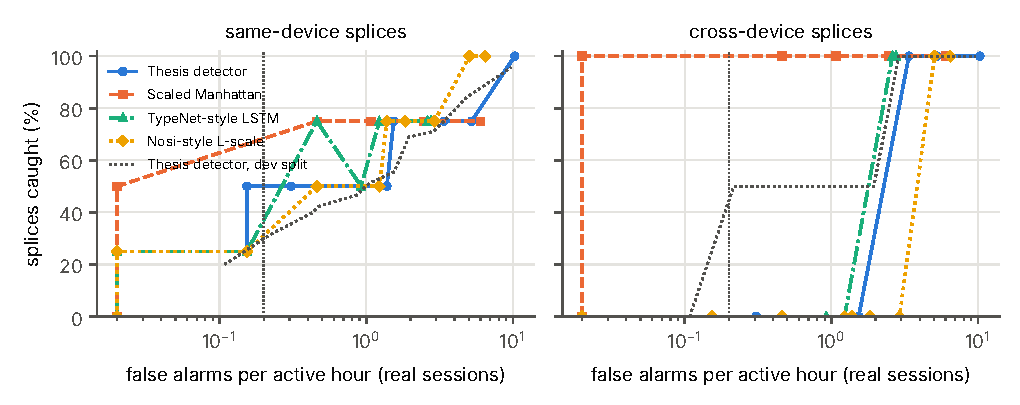
\includegraphics[width=\linewidth]{cls-detection-vs-false-alarms}
  \caption{Splices caught against false alarms per active hour on real sessions, sweeping the
    calibration target (held-out split, thresholds from dev at each target; dotted: thesis
    detector on the cross-fitted dev split). Vertical line: the frozen target, 0.2 per hour.}
  \label{fig:cls-curves}
\end{figure}

% Generated by studentide.harness.classroom_report. Do not edit by hand.
\begin{table}[ht]
  \centering\small
  \caption{RQ1 and RQ4 on the dev split, 5-fold cross-fitted: each fold's thresholds come from the other folds' students (holdout calibration, 0.2 false alarms per hour), so every number is out of sample for the thresholds. 90 real sessions of 88 students, 27.7 active hours, 45 same-device splices. Precision assumes 1 in 100 or 1 in 500 sessions contain a takeover.}
  \label{tab:cls-dev-methods}
  \resizebox{\linewidth}{!}{\begin{tabular}{@{}lrrrrrr@{}}
    \toprule
    Method & False alarms / h & Sessions flagged & Same-device caught & Delay (min) & Precision 1/100 & 1/500 \\
    \midrule
    Thesis detector (all channels) & 0.22 {\scriptsize[0.04, 0.43]} & 6\% {\scriptsize[1, 11]} & 31\% {\scriptsize[18, 45]} & 10.0 {\scriptsize[7.5, 19.5]} & 5.4\% {\scriptsize[2.7, 20.1]} & 1.1\% {\scriptsize[0.5, 4.8]} \\
    \quad identity channels only & 0.14 {\scriptsize[0.03, 0.29]} & 4\% {\scriptsize[1, 9]} & 29\% {\scriptsize[16, 43]} & 11.5 {\scriptsize[7.5, 19.5]} & 6.2\% {\scriptsize[2.8, 22.9]} & 1.3\% {\scriptsize[0.6, 5.6]} \\
    Thesis detector, deployed thresholds & 1.59 {\scriptsize[1.12, 2.06]} & 29\% {\scriptsize[20, 38]} & 64\% {\scriptsize[49, 78]} & 7.5 {\scriptsize[3.0, 10.5]} & 2.2\% {\scriptsize[1.7, 3.1]} & 0.4\% {\scriptsize[0.3, 0.6]} \\
    \midrule
    Scaled Manhattan & 0.18 {\scriptsize[0.00, 0.40]} & 3\% {\scriptsize[0, 7]} & 29\% {\scriptsize[17, 43]} & 7.5 {\scriptsize[2.5, 17.5]} & 8.0\% {\scriptsize[3.5, 100.0]} & 1.7\% {\scriptsize[0.7, 100.0]} \\
    TypeNet-style LSTM & 0.11 {\scriptsize[0.00, 0.30]} & 2\% {\scriptsize[0, 6]} & 16\% {\scriptsize[5, 27]} & 15.5 {\scriptsize[1.5, 28.8]} & 6.6\% {\scriptsize[2.0, 100.0]} & 1.4\% {\scriptsize[0.4, 100.0]} \\
    Nosi-style L-scale & 0.25 {\scriptsize[0.00, 0.64]} & 2\% {\scriptsize[0, 6]} & 13\% {\scriptsize[4, 23]} & 9.5 {\scriptsize[3.8, 13.8]} & 5.7\% {\scriptsize[2.5, 100.0]} & 1.2\% {\scriptsize[0.5, 100.0]} \\
    \bottomrule
  \end{tabular}}
\end{table}


\paragraph{What the splices leave out.} $B$ continues their own code, so build order and
the absence of a reading pause favour the process channel (\cref{sec:splicing}); its small
contribution at real-data thresholds means this bias barely touches the headline. Real
sessions may contain real switches, so the false-alarm rates are upper bounds.

\section{Synthetic pilot (phase 2 of the build)}
Before any student data, the detector was evaluated on 60 simulated typists
(\cref{ch:detector}), each with four honest 30-minute baseline sessions and
seven test sessions (A honest $\times 2$, B proxy, C takeover by a
speed-matched and by a random partner, D copying out, E paste). Twenty
typists calibrate the thresholds; the other forty are the test set.
Generated by \texttt{python -m studentide.detector.evaluate --typists 60
--seed 7}; raw results are next to each table under \texttt{ablations/}. How the code was
verified, and the development runs behind each design choice, are in
\cref{app:verification}.


\subsection*{Results}

On the synthetic test set with $W=30$\,s (\cref{tab:detection-by-condition,fig:detection-by-condition}),
a speed-matched partner taking over is caught in 72\% of sessions, with a
median delay of 80\,s after the switch and a median error of 29\,s in the
estimated switch time; with a random partner, 88\%. The identity channel
raises almost all of these alarms first. Copying out (80\%) and pasting
(78\%) are caught mostly by the process channel. The cost is 0.42 false
alarms per hour of honest work on the test typists (11\% of honest
sessions flagged at least once), twice the 0.2 per hour the thresholds were
calibrated for, a sign that 20 calibration typists are too few to set $h$
tightly. At realistic cheating rates this false-alarm level is the main
problem, which RQ4 has to address.

% Generated by studentide.detector.evaluate (seed 7, 60 typists, 30-min sessions). Do not edit by hand.
\begin{table}[ht]
  \centering\small
  \caption{Switch detection by condition on synthetic test typists ($W=30$\,s,
    $k=1/0.5$, $h=5.25/11$ for identity/process). Honest sessions: 0.42 false alarms per hour,
    10\% of honest sessions flagged at least once.}
  \label{tab:detection-by-condition}
  \resizebox{\linewidth}{!}{\begin{tabular}{@{}lrcrrrrc@{}}
    \toprule
    Condition & $n$ & Detected & Delay med.\ (s) & Delay p90 (s) & Switch err.\ (s) & Early alarms & First: id/proc \\
    \midrule
    B full proxy (matched) & 40 & 88\% & 150 & 648 & 0 & 0 & 31/4 \\
    C takeover (matched) & 40 & 75\% & 86 & 380 & 30 & 6 & 28/2 \\
    C takeover (random partner) & 40 & 88\% & 65 & 275 & 31 & 8 & 33/2 \\
    D copying out & 40 & 50\% & 448 & 874 & 37 & 12 & 3/17 \\
    E paste & 40 & 82\% & 441 & 821 & 40 & 8 & 4/29 \\
    \bottomrule
  \end{tabular}}
\end{table}


\begin{figure}[ht]
  \centering
  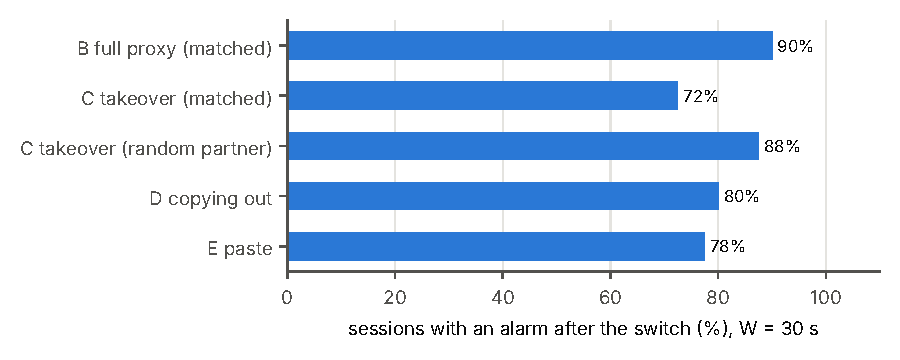
\includegraphics[width=0.8\linewidth]{detection-by-condition}
  \caption{Synthetic sessions with an alarm after the switch, by condition.}
  \label{fig:detection-by-condition}
\end{figure}

\section{Ablations}
\paragraph{Window length.} Longer windows separate a single window better
(balanced accuracy 0.80 at 30\,s, 0.85 at 150\,s; Nosi reports about 80\% at
150\,s for composing vs.\ transcribing \cite{lueder2026nosi}), but the CUSUM
already accumulates evidence over short windows, so for takeovers short
windows win: median delay 80\,s at 30\,s against 7 minutes at 150\,s, while
the detection rate does not improve (60--78\% at every length). Copying out
is a smaller shift and gains from longer windows: 80\% at 30\,s, 90--100\%
at 90\,s and above. This suggests running the two channels at different
window lengths (\cref{tab:ablation-window-length,fig:window-length}).

\begin{figure}[ht]
  \centering
  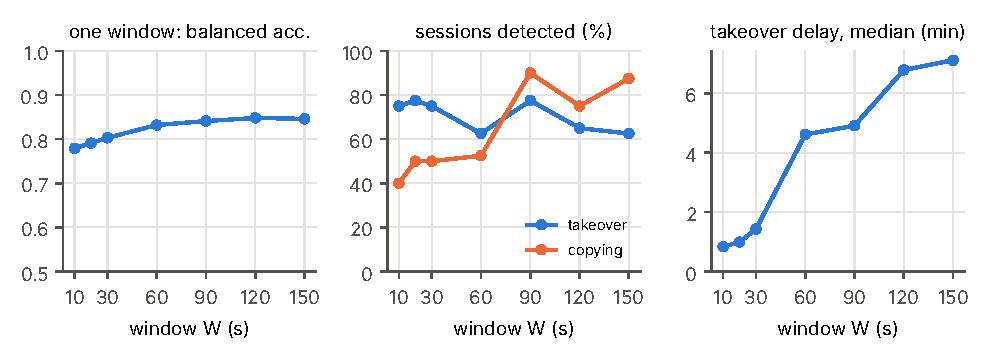
\includegraphics[width=\linewidth]{window-length-tradeoff}
  \caption{Window-length trade-off on synthetic sessions.}
  \label{fig:window-length}
\end{figure}

\paragraph{Features and design choices} (\cref{tab:ablation-feature-groups}).
The rhythm group carries the identity channel: without it, matched
takeovers drop from 72\% to 38\%. Focus and paste features carry copying
and pasting (without focus, copying drops to 8\%).

The first version measured build order per edit (share of edits away from
the end of the file, caret jumps per minute). Those numbers swing from one
window to the next, inflating the process channel's spread, and removing
them raised copying detection from 50\% to 95\%. They were replaced by two
line-level measures over the trailing five minutes: the share of new code
lines written above existing code, and the number of block headers still
without a body (\cref{tab:features}). The replacement was chosen on a
separate development population (seed 3) and the reported run was made
once afterwards. On the test set copying detection rose from 50\% (old
features, row ``Old build order'') to 80\% with the same false-alarm rate.
Dropping build order altogether still detects more copying (95\%), at
slightly more false alarms (0.47 per hour); on simulated data the feature
mostly adds a habit that transcription does not change, so whether it
earns its place has to be decided on real sessions.

A single channel with equal weights detects only 60\% of matched
takeovers; a single ICC-weighted channel detects 70\% but almost no copying
or pasting (10\% each), which motivated the two channels. The Nosi-style
detector (L-scale only) catches 18\% of takeovers, as expected for a
measure designed for composing vs.\ transcribing. Keeping comment
keystrokes apart made no difference on synthetic data (72\% either way),
unsurprising because simulated comments differ from code by a single
offset; this needs re-testing on real sessions.

\section{Evaluation harness: detector against baselines (synthetic)}
\label{sec:rq1-harness}
The pilot above tuned and reported on one population of 60. The evaluation
harness (\cref{sec:protocol}) replaces it with the protocol the study data will
go through: a fresh simulated population of 120 students (seed 2026, never used
before), 84 dev and 36 test students split by hashed id, every choice made on dev
with 5-fold cross-fitting, then the test students scored once per frozen
configuration (\texttt{thesis/evaluation/test-ledger.jsonl} records every run:
two so far, the configuration of phase 4 and the one with key-pair timing
below, each scored exactly once). Each
student has 8 baseline sessions, of which the first 4 form the baseline, and the
same seven test sessions as in the pilot.

\paragraph{Choices made on dev.} Thresholds are calibrated on the
\emph{pooled} source (other students' staged honest sessions plus every
student's own baseline sessions scored leave-one-session-out; see
\cref{sec:calibration-finding}). The process channel runs on 90\,s windows
while the identity channel keeps 30\,s, and both channels use the population
prior (\cref{sec:short-baselines}); together these raised mean detection over
the five non-honest conditions from 73\% to 85\% on dev
(\cref{tab:harness-tuning}). Each baseline got its own best alarm rule and $k$
on dev; all chose a CUSUM, none the per-window threshold.

The first test run (configuration of phase 4, two channels) found scaled
Manhattan ahead on speed-matched takeovers, 89\% against 64\%. Scaled
Manhattan compares individual digraphs, whereas the identity channel only had
grouped ones (alternating hands, into the space bar, \dots). Per-key-pair
timing was therefore added (\cref{sec:detector-channels}) and its use chosen on
dev, without looking at the test students again: inside the identity
channel at weight 0.5, 1 or 2, or as a channel of its own with $k\in\{0.25,
0.5, 1\}$ and 20, 40 or 80 pairs. A channel of its own with $k=0.5$ and 80
pairs was best, raising mean detection on dev from 85\% to 92\% (matched
takeovers 57\% $\to$ 75\%, proxies 77\% $\to$ 95\%) at the same false-alarm
rate; inside the identity channel the pairs added at most 6 points on matched
takeovers. This became the second frozen configuration, and the test
students were scored with it once. The numbers below are from that run.

\paragraph{Results on the test students} (\cref{tab:harness-methods,tab:harness-conditions,fig:harness-curves}).
At the frozen operating point the thesis detector catches all copying-out and
pasting sessions (delays of about 4.5 and 3 minutes), 89\% of full proxies,
83\% of takeovers by a random classmate and 86\% (95\% interval 75--97\%) by a
speed-matched one, with a median delay of 4.6 minutes. Honest sessions see
0.19 false alarms per hour (interval 0.06--0.39; 7\% of honest sessions with
any alarm), on the 0.2 target. Over all non-honest sessions it detects 92\%,
against 53\% for scaled Manhattan, 39\% for the TypeNet-style model and 47\%
for the Nosi-style measure. With the two-channel configuration the same test
students gave 64\% of matched takeovers, 69\% of proxies, 83\% overall and
0.28 false alarms per hour. The key-pair channel fires first on about half of
the caught proxies and matched takeovers (16 of 32 and 16 of 31), the
rhythm channel on most of the random-partner takeovers (21 of 30), whose
overall speed already differs.

Scaled Manhattan is still slightly ahead on matched takeovers (89\% against
86\%, well inside each other's intervals) and faster (3.5 against 4.6 minutes),
but it is blind to copying and pasting (6\% and 8\%), because the same hands
keep typing. The TypeNet-style model separates single windows almost as well
(AUC 0.83 against 0.86) but trained on only 84 students it does not reach the
hand-built features. The Nosi-style L-scale, designed for transcription,
catches two thirds of copying but few switches.

% Generated by studentide.harness (synthetic:synth-v1-n120-s2026-b8-m30, test split, 36 students). Do not edit by hand.
\begin{table}[ht]
  \centering\small
  \caption{RQ1 on the synthetic test students: the thesis detector against the baselines, each with its alarm threshold calibrated on dev students for $\le 0.2$ false alarms per honest hour (alarm rule, $k$ and window chosen on dev, \cref{tab:harness-tuning}). Detected = alarm after the switch; delay = median for matched takeovers; Win.\ AUC = one window, honest vs.\ typed by another person.}
  \label{tab:harness-methods}
  \resizebox{\linewidth}{!}{\begin{tabular}{@{}lcccccccrr@{}}
    \toprule
    Method & Win.\ AUC & Proxy & Takeover & Take.\ (rand.) & Copying & Paste & Delay (s) & FA/h & Flagged \\
    \midrule
    Two-channel CUSUM & 0.86 & 69\% & 64\% & 81\% & 100\% & 100\% & 295 & 0.28 & 7\% \\
    Scaled Manhattan & 0.86 & 83\% & 89\% & 81\% & 6\% & 8\% & 208 & 0.30 & 12\% \\
    TypeNet-style LSTM & 0.83 & 56\% & 56\% & 72\% & 14\% & 0\% & 293 & 0.33 & 10\% \\
    Nosi-style L-scale & 0.67 & 58\% & 53\% & 44\% & 67\% & 11\% & 178 & 0.25 & 7\% \\
    \bottomrule
  \end{tabular}}
\end{table}

% Generated by studentide.harness (synthetic:synth-v1-n120-s2026-b8-m30, test split, 36 students). Do not edit by hand.
\begin{table}[ht]
  \centering\small
  \caption{Thesis detector by condition on the synthetic test students ($k=1/0.5$, $h=19.25/7.25$ for identity/process, 95\% student-bootstrap intervals). Honest sessions: 0.28 {\scriptsize[0.06, 0.61]} false alarms per hour, 7\% {\scriptsize[1, 12]} of honest sessions with at least one alarm.}
  \label{tab:harness-conditions}
  \resizebox{\linewidth}{!}{\begin{tabular}{@{}lrlrrrrc@{}}
    \toprule
    Condition & $n$ & Detected & Delay med.\ (s) & Delay p90 (s) & Switch err.\ (s) & Early alarms & First: id/proc \\
    \midrule
    B full proxy (matched) & 36 & 69\% {\scriptsize[53, 83]} & 360 {\scriptsize[210, 450]} & 738 & 0 & 0 & 17/8 \\
    C takeover (matched) & 36 & 64\% {\scriptsize[47, 78]} & 295 {\scriptsize[212, 423]} & 723 & 26 & 0 & 21/2 \\
    C takeover (random partner) & 36 & 81\% {\scriptsize[67, 92]} & 182 {\scriptsize[144, 251]} & 499 & 36 & 1 & 26/3 \\
    D copying out & 36 & 100\% {\scriptsize[100, 100]} & 261 {\scriptsize[239, 275]} & 330 & 59 & 0 & 1/35 \\
    E paste & 36 & 100\% {\scriptsize[100, 100]} & 170 {\scriptsize[131, 178]} & 241 & 62 & 0 & 0/36 \\
    \bottomrule
  \end{tabular}}
\end{table}


\begin{figure}[ht]
  \centering
  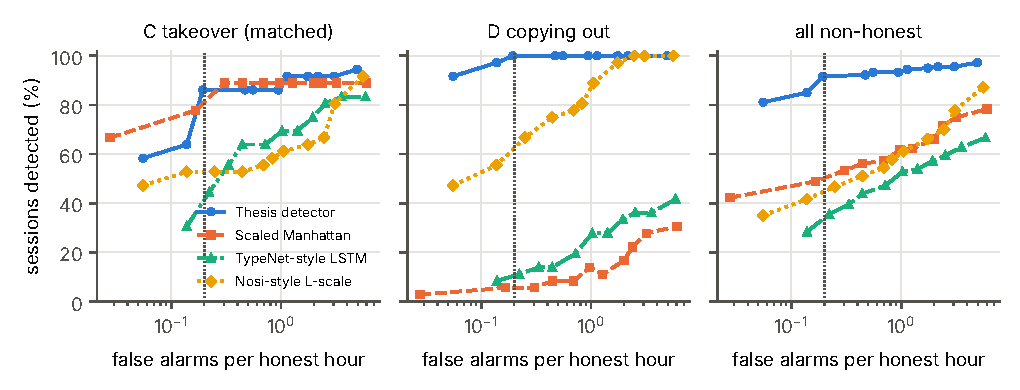
\includegraphics[width=\linewidth]{harness-detection-vs-false-alarms}
  \caption{Detection against false alarms per honest hour on the synthetic test
    students, sweeping the calibration target (dotted line: 0.2 per hour).}
  \label{fig:harness-curves}
\end{figure}

\subsection{Calibrating the threshold}
\label{sec:calibration-finding}
The pilot's thresholds, set on 20 students' staged honest sessions, gave twice
the target false-alarm rate. The harness reproduces this on dev: with 20
calibration students the \emph{holdout} source gives 0.43 false alarms per hour
for a 0.2 target, and even 68 students give 0.30
(\cref{tab:harness-calibration,fig:harness-calibration}). Each student
contributes only two honest test sessions, so $h$ is set by a handful of
alarms. Scoring every student's own baseline sessions leave-one-session-out
(\emph{self}) needs no staged sessions and quadruples the honest hours; it hits
the target with 20 students (0.20) and errs on the conservative side with more.
The pooled source was the closest on average and is the frozen choice; on the
unseen test students (key-pair configuration) it gives 0.19, self alone 0.19 and holdout alone 0.28. In
the study this means every enrolled student's baseline weeks double as
calibration data, so $h$ need not wait for staged sessions.

\begin{figure}[ht]
  \centering
  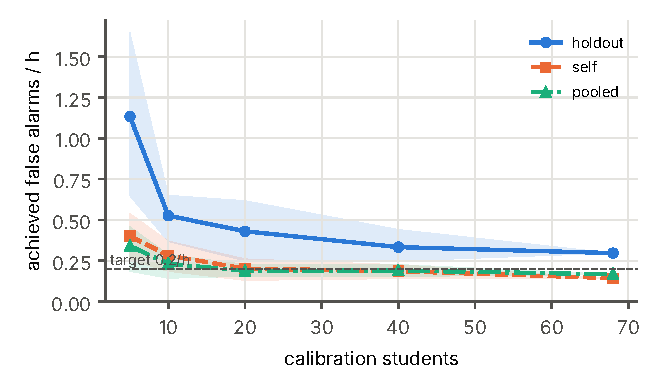
\includegraphics[width=0.65\linewidth]{harness-calibration}
  \caption{Achieved false alarms per hour against calibration students (dev,
    mean and 10--90th percentile over 20 draws), target 0.2 per hour.}
  \label{fig:harness-calibration}
\end{figure}

\subsection{Short baselines}
\label{sec:short-baselines}
A student who missed lab weeks has a thin baseline, and the review dashboard
showed baseline-week sessions raising moments against a leave-one-out baseline
of one or two sessions. The population prior shrinks a student's per-feature
spread and honest score level towards the population's, as if the population
were worth two more sessions. On dev (\cref{tab:harness-baseline-length,fig:harness-baseline-length})
it makes two baseline sessions nearly as good as four: copying 100\% against
70\% without it, matched takeovers 69\% against 66\% (75\% with four). With one
session it cuts honest sessions flagged from 14\% to 11\% (0.32 to 0.21 false
alarms per hour) but, since key-pair timing was added, also costs matched
takeovers (51\% $\to$ 37\%): the prior widens the spread of 80 per-pair
features the student has barely been measured on. With six or eight sessions
it no longer matters much. (Numbers from the second dev run, with key pairs;
the first run, without them, is in the brain log.)

\begin{figure}[ht]
  \centering
  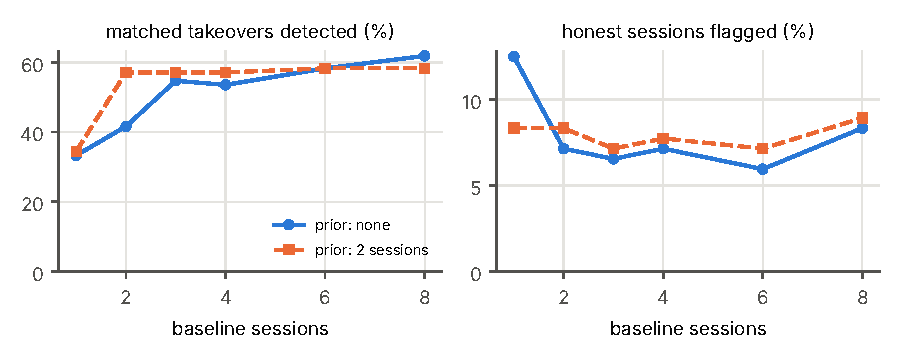
\includegraphics[width=0.8\linewidth]{harness-baseline-length}
  \caption{Baseline length with and without the population prior (dev).}
  \label{fig:harness-baseline-length}
\end{figure}

\subsection{Ablations on dev}
The harness ablations (\cref{app:ablations}) confirm the pilot's design on
new students with cross-fitting. Removing the key-pair channel costs 18 points
on matched takeovers (75\% $\to$ 57\%) and 18 on proxies; not subtracting the
window's own pace costs little on synthetic data (one point overall, more
false alarms), and letting the key-pair channel replace the rhythm channel
loses 14 points on matched takeovers, so both typing channels are kept.
With key-pair timing the population prior no longer helps with a single
baseline session (matched takeovers 51\% without it, 37\% with), though it
still helps copying (70\% $\to$ 96\%) and from two sessions on.
Rhythm still matters on top of the key pairs (matched takeovers 75\% $\to$ 57\%
and window AUC 0.86 $\to$ 0.68 without it) and focus carries copying (99\%
$\to$ 5\%). The accumulating CUSUM matters: a per-window threshold at the same
false-alarm rate catches 29\% of matched takeovers and 24\% of copying. One
ICC-weighted channel misses copying and pasting (4\%, 5\%). Window length shows
the split the pilot suggested: matched takeovers are caught soonest with short
windows (152\,s delay at 10\,s), copying best with 90\,s and longer (93\%),
hence the typing channels at 30\,s and process at 90\,s. The line-level
build-order features earn a small place (without them proxies drop from 95\%
to 90\%), whereas the old per-edit version cuts copying to 77\%. Keeping
comment keystrokes apart still changes nothing on simulated data.

\section{Summary}
RQ1 asked how well a change of author can be detected in real classwork. With the live
detector settings and thresholds set on real dev sessions for 0.2 false alarms per active
hour, about a third of spliced takeovers are caught (31\%, 18--45\% on 45 dev splices),
typically ten minutes after the switch, and the rate held on unseen students (0.15 per hour on
the held-out split). Detection can be bought with false alarms (64\% at 1.59 per hour, the
deployed setting), but not cheaply. The identity channels do most of the work, and a plain
per-key timing comparison does about as well, so the contribution of this design lies less in
a stronger detector than in measuring honestly what one can do in class. The held-out split
is too small to confirm detection (4 splices); because every session from 24 November is held
out, it grows with the term, and a final test run on it is planned and will be logged.
